%\section{Linear Forms}
\begin{python0}
from solutions import *; clear() 
\end{python0}

Now we use power series to solve some combinatorial / discrete problems.
Before we begin, let's step back and look at the big picture.

In many combinatorial problems (including problems from CS), one is usually
interested in understanding not just a number such as
\lq\lq how many steps do you need to sort these 1000 numbers if we use 
algorithm $X$?''
Instead we're usually interested in a family of related problems:
\lq\lq how many steps do you need to sort these $n$ numbers if we use 
algorithm $X$?''
If $t_n$ is the number of steps, then in fact we're looking at not just
one number but an infinite sequence of numbers:
\[
t_0, t_1, t_2, t_3, \ldots
\]

So far we've been studying such numbers individually, or
in the case of mathematical induction, we're looking at $t_{n+1}$
from the point of view of $t_n$.
Note also that although we've been proving theorems such as
\[
1 + 2 + \cdots + n = \frac{n(n+1)}{2}
\]
using mathematical induction, you should realize by now that
mathematical induction requires us to start with a 
hypothesis:
You have to do some experiments to come up with a plausible
formula or fact before you can apply induction to prove
the correctness of your conjecture.

The technique and power of the power series is that instead of
looking at numbers one at a time, we will build a single object to study.
So instead of studying a sequence of infinite things:
\[
t_0, t_1, t_2, t_3, \ldots
\]
one at a time, we will combine them together to form a power series:
\[
t(x) = \sum_{n=0}^\infty t_n x^n
\]

We say that 
\[
t(x) = \sum_{n=0}^\infty t_n x^n
\]
is the \defone{ordinary generating function} of the sequence
\[
t_0, t_1, t_2, t_3, \ldots
\]

Of course since I'm calling this the \textit{ordinary} generating
function, you would expect other types of generating functions.
That is in fact the case although the ordinary is the most common.
Our generating function is built from $t_0, t_1, t_2, \ldots$
together with $x^0, x^1, x^2, \ldots$.
In general it's possible to talk about generating functions 
with a collection of kernel functions $K_0(x), K_1(x), K_2(x), \ldots$:
\[
\sum_{n=0}^\infty t_n K_n(x)
\]
Different kernel functions solve different problems.
Anyway let's get back to the ordinary case.

One extremely important thing about polynomial multiplication
is that it is a combinatorial operation.
For instance look at this:
\[
(1 + x + x^2 + x^3 + x^4)
(1 + x + x^2 + x^3)
\]
Of course you know how to multiply two polynomials.
But notice that each term in the product looks like this
\[
x^i x^j
\]
where $x^i$ is from $1 + x + x^2 + x^3 + x^4$ and 
$x^i$ is from $1 + x + x^2 + x^3$.
In particular look at the term with $x$-power of $x^3$.
The following lists all the pairs (underlined) that will contribute
towards the $x^3$ term in the final product:
\begin{align*}
&(\underline{1} + x + x^2 + x^3 + x^4)(1 + x + x^2 + \underline{x^3}) \\
&(1 + \underline{x} + x^2 + x^3 + x^4)(1 + x + \underline{x^2} + x^3) \\
&(1 + x + \underline{x^2} + x^3 + x^4)(1 + \underline{x} + x^2 + x^3) \\
&(1 + x + x^2 + \underline{x^3} + x^4)(\underline{1} + x + x^2 + x^3) \\
\end{align*}
i.e. the $x^3$ term is
\[
x^0x^3 + x^1x^2 + x^2x^1 + x^3x^0 = 4x^3
\]
The multiplication process is combinatorial in the sense that
one has to \textit{choose} terms.
In this case,
I have to choose a term from the first polynomial and
a term from the second.

Now what if I multiply the following:
\[
(1 + x + x^3 + x^4)
(1 + x + x^2 + x^3)
\]
Note that $x^2$ is missing from the first polynomial.
What is the term with $x$-power of $x^3$?
\begin{align*}
&(\underline{1} + x + x^3 + x^4)(1 + x + x^2 + \underline{x^3}) \\
&(1 + \underline{x} + x^3 + x^4)(1 + x + \underline{x^2} + x^3) \\
&(1 + x + \underline{x^3} + x^4)(\underline{1} + x + x^2 + x^3) \\
\end{align*}
In this case I have
\[
x^0x^3 + x^1x^2 + x^3x^0 = 3x^3
\]

Now look at the above simple computations very carefully.
In the first example, do you see that
\[
\text{ The 4 in 4$x^3$ comes from } 3 = 0+3, 1+2, 2+1, 3+0
\]
and the second example
\[
\text{ The 3 in $3x^3$ comes from } 3 = 0+3, 1+2, 3+0
\]
If you don't see that, you should go over the examples above again.

If I want to count the number of ways to select $a$ from $\{0, 1, 2, 3, 4\}$
and $b$ from $\{0, 1, 2, 3\}$ such that
\[
a + b = 3
\]
then all I need is to compute the coefficient of $x^3$ in 
\[
(x^0 + x^1 + x^2 + x^3 + x^4)
(x^0 + x^1 + x^2 + x^3)
\]
Of course the first polynomial is created from $\{0,1,2,3,4\}$:
\[
(x^0 + x^1 + x^2 + x^3 + x^4) = \sum_{n \in \{0, 1, 2, 3, 4\}} x^n
\]
Likewise the second polynomial is created from $\{0, 1, 2, 3\}$
resulting in 
\[
(x^0 + x^1 + x^2 + x^3) = \sum_{n \in \{0, 1, 2, 3\}} x^n
\]

On the other hand if the $a$ must be chosen from $\{1, 3, 5\}$ 
and $b$ is chosen from $\{0,1,2,3\}$ then the 
number of ways to select $a$ and $b$ such that $a + b = 3$
is the coefficient of 
\[
(x^1 + x^3 + x^5)(x^0 + x^1 + x^2 + x^3)
\]
See that?


\newpage
\begin{ex}
  Let $A = \{2, 3, 4, 5, 6, 7 \}$ and $B = \{ 1, 3, 5, 7, 9\}$.
  \begin{enumerate}[nosep,label=(\alph*)]
  \item
    How many possible ways are there to choose $a$ from $A$ and $b$ from $B$
    such that
    \[
    a + b = 8
    \]
    (List all the possible $(a,b)$'s.)
    Compute the coefficient of $x^8$ in the product
    \[
    (x^2+x^3+x^4+x^5+x^6+x^7)(x+x^3+x^5+x^9)
    \]
  \item
    What is the number of ways to choose $a$ from $A$ and $b$ from $B$
    such that 
    \[
    a + b = 5
    \]
    What is the coefficient of $x^5$ in the above product of polynomials?
  \end{enumerate}
\end{ex}



\newpage
\begin{ex}
How many ways are there to choose $a$ and $b$ such that
\[
a + b = 6
\]
such that $a \geq 0$ is an integer, and
$b \geq 0$ is an even integer.
Compute this number in two different ways:
one by listing all possible $(a, b)$ and another way by 
computing the coefficient of $x^6$ of the product
of two polynomials.
Now change 6 to any positive integer $n$ and solve the
problem in general.
\end{ex}


\newpage
\begin{ex}
How many ways are there to choose $a$ and $b$ such that
\[
a + b = 6
\]
such that $a \geq 2$ is an integer, and
$b \geq 0$ is an odd integer.
Again compute this number in two different ways:
one by listing all possible $(a, b)$ and another way by 
computing the coefficient of $x^6$ of the product
of two polynomials.
Now change 6 to any positive integer $n$ and solve the
problem in general.
\end{ex}


\newpage
\begin{ex}
Let $n \geq 0$.
How many ways are there to choose $a$ and $b$ such that
\[
a + b + c + d = n
\]
such that $a, b, c \geq 0$ are integers 
and $2 \leq d \leq 100$ are integers. 
\end{ex}



\newpage
\begin{ex}
How many ways are there to choose $a$ and $b$ such that
\[
a + b + c + d = 6
\]
such that $a \geq 2$ is an integer,
$b \geq 0$ is an odd integer,
and both $c \geq 0$ and $d \geq 0$ are integers. 
Again compute this number in two different ways:
one by listing all possible $(a, b)$ and another way by 
computing the coefficient of $x^6$ of the product
of two polynomials.
Now change 6 to any positive integer $n$ and solve the
problem in general.
\end{ex}



\newpage
\begin{ex}
How many solutions are there to
the following problem:
\begin{align*}
a + 2b + 3c + d= 100
\end{align*}
where $a, b, c, d$ are positive integers (including $0$).
What if $100$ is any positive integer $n$?
\end{ex}



\newpage
\begin{ex}
How many solutions are there to
the following problem:
\begin{align*}
a + 2b + 3c + d= 100
\end{align*}
where $a, b, c, d$ are positive integers (including $0$)
and $a \geq 2$.
What if $100$ is any positive integer $n$?
\end{ex}

\newpage
\begin{ex}
How many solutions are there to 
the following problem:
\begin{align*}
a + 2b + 3c + d = 100
\end{align*}
where $a, b, c, d$ are positive integers (including $0$)
and $2 \leq d \leq 5$.
What if $100$ is any positive integer $n$?
\end{ex}

\newpage
\subsection*{Solutions}

\newpage
\section*{Solutions}
Solution to Exercise \ref{ex:dfa0}\labeltext{}{sol:dfa0}.

\tinysidebar{\debug{exercises/{dfa0/answer.tex}}}

    Solution not provided.
    

\newpage

Solution to Exercise \ref{ex:dfa1}\labeltext{}{sol:dfa1}.

\tinysidebar{\debug{exercises/{dfa1/answer.tex}}}
  The ID computation is
  \begin{align*}
    (q_0, aba)
    &\vdash (\delta(q_0, a), ba) = (q_0, ba) \\ 
    &\vdash (\delta(q_0, b), a) = (q_1, a) \\
    &\vdash (\delta(q_1, a), \ep) = (q_0, \ep)
  \end{align*}
  $q_0$ is not an accept state. Therefore $aba$ is not accepted.


\newpage

Solution to Exercise \ref{ex:dfa4}\labeltext{}{sol:dfa4}.

\tinysidebar{\debug{exercises/{dfa4/answer.tex}}}

    Solution not provided.
    

\newpage

Solution to Exercise \ref{ex:dfa5}\labeltext{}{sol:dfa5}.

\tinysidebar{\debug{exercises/{dfa5/answer.tex}}}

    Solution not provided.
    

\newpage

Solution to Exercise \ref{ex:implementing-a-single-dfa0}\labeltext{}{sol:implementing-a-single-dfa0}.

\tinysidebar{\debug{exercises/{implementing-a-single-dfa0/answer.tex}}}

    Solution not provided.
    

\newpage

Solution to Exercise \ref{ex:nfastatediag0}\labeltext{}{sol:nfastatediag0}.

\tinysidebar{\debug{exercises/{nfastatediag0/answer.tex}}}

    Solution not provided.
    

\newpage

Solution to Exercise \ref{ex:nfastatediag1}\labeltext{}{sol:nfastatediag1}.

\tinysidebar{\debug{exercises/{nfastatediag1/answer.tex}}}

    Solution not provided.
    

\newpage

Solution to Exercise \ref{ex:nfastatediag2}\labeltext{}{sol:nfastatediag2}.

\tinysidebar{\debug{exercises/{nfastatediag2/answer.tex}}}

    Solution not provided.
    

\newpage

Solution to Exercise \ref{ex:nfastatediag3}\labeltext{}{sol:nfastatediag3}.

\tinysidebar{\debug{exercises/{nfastatediag3/answer.tex}}}

    Solution not provided.
    

\newpage

Solution to Exercise \ref{ex:nfastatediag4}\labeltext{}{sol:nfastatediag4}.

\tinysidebar{\debug{exercises/{nfastatediag4/answer.tex}}}

    Solution not provided.
    

\newpage

Solution to Exercise \ref{ex:nfastatediag5}\labeltext{}{sol:nfastatediag5}.

\tinysidebar{\debug{exercises/{nfastatediag5/answer.tex}}}

    Solution not provided.
    

\newpage

Solution to Exercise \ref{ex:nfastatediag6}\labeltext{}{sol:nfastatediag6}.

\tinysidebar{\debug{exercises/{nfastatediag6/answer.tex}}}

    Solution not provided.
    

\newpage

Solution to Exercise \ref{ex:nfastatediag7}\labeltext{}{sol:nfastatediag7}.

\tinysidebar{\debug{exercises/{nfastatediag7/answer.tex}}}

    Solution not provided.
    

\newpage

Solution to Exercise \ref{ex:nfastatediag8}\labeltext{}{sol:nfastatediag8}.

\tinysidebar{\debug{exercises/{nfastatediag8/answer.tex}}}

    Solution not provided.
    

\newpage

Solution to Exercise \ref{ex:nfastatediag9}\labeltext{}{sol:nfastatediag9}.

\tinysidebar{\debug{exercises/{nfastatediag9/answer.tex}}}

    Solution not provided.
    

\newpage

Solution to Exercise \ref{ex:nfastatediag10}\labeltext{}{sol:nfastatediag10}.

\tinysidebar{\debug{exercises/{nfastatediag10/answer.tex}}}

    Solution not provided.
    

\newpage

Solution to Exercise \ref{ex:nfastatediag11}\labeltext{}{sol:nfastatediag11}.

\tinysidebar{\debug{exercises/{nfastatediag11/answer.tex}}}

    Solution not provided.
    

\newpage

Solution to Exercise \ref{ex:nfastatediag12}\labeltext{}{sol:nfastatediag12}.

\tinysidebar{\debug{exercises/{nfastatediag12/answer.tex}}}

    Solution not provided.
    

\newpage

Solution to Exercise \ref{ex:nfastatediag13}\labeltext{}{sol:nfastatediag13}.

\tinysidebar{\debug{exercises/{nfastatediag13/answer.tex}}}

    Solution not provided.
    

\newpage

Solution to Exercise \ref{ex:nfa0}\labeltext{}{sol:nfa0}.

\tinysidebar{\debug{exercises/{nfa0/answer.tex}}}
The formal definition of this NFA is $(\Sigma, Q, q_0, \delta, F)$ where
\begin{tightlist}
\li $\Sigma = \{a,b\}$
\li $Q = \{q_0\}$
\li $\delta$ is the function
\[
\delta : Q \times \Sigma_\epsilon \rightarrow P(Q)
\]
given by
\begin{align*}
  \delta(q_0, \epsilon) &= \{\} \\
  \delta(q_0, a) &= \{\} \\
  \delta(q_0, b) &= \{\} 
\end{align*}
\end{tightlist}


\newpage

Solution to Exercise \ref{ex:nfa1}\labeltext{}{sol:nfa1}.

\tinysidebar{\debug{exercises/{nfa1/answer.tex}}}

    Solution not provided.
    

\newpage

Solution to Exercise \ref{ex:nfa2}\labeltext{}{sol:nfa2}.

\tinysidebar{\debug{exercises/{nfa2/answer.tex}}}

    Solution not provided.
    

\newpage

Solution to Exercise \ref{ex:nfa3}\labeltext{}{sol:nfa3}.

\tinysidebar{\debug{exercises/{nfa3/answer.tex}}}

    Solution not provided.
    

\newpage

Solution to Exercise \ref{ex:nfa4}\labeltext{}{sol:nfa4}.

\tinysidebar{\debug{exercises/{nfa4/answer.tex}}}

    Solution not provided.
    

\newpage

Solution to Exercise \ref{ex:nfa5}\labeltext{}{sol:nfa5}.

\tinysidebar{\debug{exercises/{nfa5/answer.tex}}}

    Solution not provided.
    

\newpage

Solution to Exercise \ref{ex:dfa-as-powerful-as-nfa0}\labeltext{}{sol:dfa-as-powerful-as-nfa0}.

\tinysidebar{\debug{exercises/{dfa-as-powerful-as-nfa0/answer.tex}}}
Here's the solution.
Let $\delta$ denote the transition function of $N$.
Note that 
\begin{align*}
  \delta(q_0, \epsilon) = \{\} \\
  \delta(q_0, a) = \{\} \\
  \delta(q_0, b) = \{\} 
\end{align*}
First of all the states are labeled as all the subsets of $\{q_0\}$.


\begin{center}
\begin{tikzpicture}[>=triangle 60,shorten >=0.5pt,node distance=2cm,auto,initial text=, double distance=2pt]
\node[state] (A) at (  0,  0) {$\{q_0\}$};
\node[state] (B) at (  3,  0) {$\{\}$};

\path[->]

;
\end{tikzpicture}
\end{center}
    


The start state is the $\epsilon$-closure of $\{q_0\}$.
However in $N$, there are no $\epsilon$--transitions out of 
$q_0$.
So the $\epsilon$-closure of $\{q_0\}$ is in fact $\{q_0\}$, i.e.
$\overline{\{q_0\}} = \{q_0\}$
The $\DFA$ is now this:


\begin{longtable}{|r||r|r|r|r|r|}
\hline 
         & $w_1$ & $w_2$ & $w_3$ & $w_4$ & $\ldots$ \\ \hline \hline 
$M_1$    &       &       &       &       &          \\ \hline 
$M_2$    &       &       &       &       &          \\ \hline 
$M_3$    &       &       &       &       &          \\ \hline 
$M_4$    &       &       &       &       &          \\ \hline 
$\ldots$ &       &       &       &       &          \\ \hline 
\end{longtable}
        


Now I will compute the $a$--transition of the state $\{q_0\}$.
Let $\delta^\DFA$ denote the transition function of the $\DFA$
that we're building.
Then
\begin{align*}
\delta( \{q_0, a\} ) 
&= \overline{ \bigcup_{q \in \{q_0\}} \delta(q, a)} \\
&= \overline{ \delta(q_0, a) } \\
&= \overline{ \emptyset } \\
&= \emptyset
\end{align*}
The (incomplete) $\DFA$ now looks like this:


\begin{longtable}{|r||r|r|r|r|r|}
\hline 
         & $w_1$ & $w_2$ & $w_3$ & $w_4$ & $\ldots$ \\ \hline \hline 
$M_1$    & 0     & 0     & 1     & 0     & ...      \\ \hline 
$M_2$    & 1     & 0     & 1     & 1     & ...      \\ \hline 
$M_3$    & 0     & 1     & 1     & 1     & ...      \\ \hline 
$M_4$    & 1     & 0     & 1     & 1     & ...      \\ \hline 
$\ldots$ &       &       &       &       &          \\ \hline 
\end{longtable}
        


Using the same reasoning we have

\begin{center}
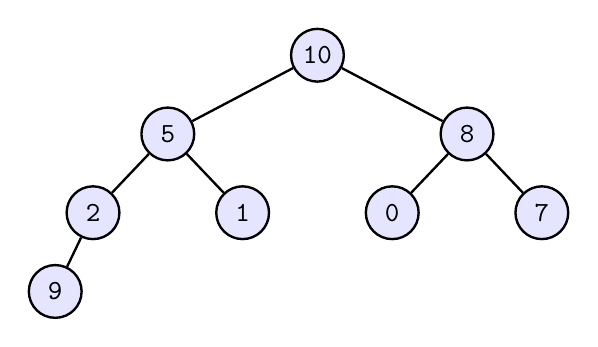
\begin{tikzpicture}

\fill[blue!10] (0.0, 0.0) circle (0.35);
\node [line width=0.03cm,black,minimum size=0.6699999999999999cm,draw,circle] at (0.0,0.0)(10){};\draw (0.0, 0.0) node[color=black] {\texttt{10}};
\fill[blue!10] (-1.9, -1.0) circle (0.35);
\node [line width=0.03cm,black,minimum size=0.6699999999999999cm,draw,circle] at (-1.9,-1.0)(5){};\draw (-1.9, -1.0) node[color=black] {\texttt{5}};
\fill[blue!10] (1.9, -1.0) circle (0.35);
\node [line width=0.03cm,black,minimum size=0.6699999999999999cm,draw,circle] at (1.9,-1.0)(8){};\draw (1.9, -1.0) node[color=black] {\texttt{8}};
\fill[blue!10] (-2.85, -2.0) circle (0.35);
\node [line width=0.03cm,black,minimum size=0.6699999999999999cm,draw,circle] at (-2.85,-2.0)(2){};\draw (-2.85, -2.0) node[color=black] {\texttt{2}};
\fill[blue!10] (-0.95, -2.0) circle (0.35);
\node [line width=0.03cm,black,minimum size=0.6699999999999999cm,draw,circle] at (-0.95,-2.0)(1){};\draw (-0.95, -2.0) node[color=black] {\texttt{1}};
\fill[blue!10] (0.95, -2.0) circle (0.35);
\node [line width=0.03cm,black,minimum size=0.6699999999999999cm,draw,circle] at (0.95,-2.0)(0){};\draw (0.95, -2.0) node[color=black] {\texttt{0}};
\fill[blue!10] (2.85, -2.0) circle (0.35);
\node [line width=0.03cm,black,minimum size=0.6699999999999999cm,draw,circle] at (2.85,-2.0)(7){};\draw (2.85, -2.0) node[color=black] {\texttt{7}};
\fill[blue!10] (-3.33, -3.0) circle (0.35);
\node [line width=0.03cm,black,minimum size=0.6699999999999999cm,draw,circle] at (-3.33,-3.0)(9){};\draw (-3.33, -3.0) node[color=black] {\texttt{9}};\draw[line width=0.03cm,black] (10) to  (5);
\draw[line width=0.03cm,black] (10) to  (8);
\draw[line width=0.03cm,black] (5) to  (2);
\draw[line width=0.03cm,black] (5) to  (1);
\draw[line width=0.03cm,black] (8) to  (0);
\draw[line width=0.03cm,black] (8) to  (7);
\draw[line width=0.03cm,black] (2) to  (9);
\end{tikzpicture}

\end{center}



It's easy to see that in the DFA, the $a$--
and $b$--transitions from the state $\{\}$ goes back to itself.
Therefore the completed DFA is this:


\begin{center}
\begin{tikzpicture}[>=triangle 60,shorten >=0.5pt,node distance=2cm,auto,initial text=, double distance=2pt]
\node[state,initial] (A) at (  0,  0) {$\{q_0\}$};
\node[state] (B) at (  3,  0) {$\{\}$};

\path[->]
(A) edge [bend left=0,pos=0.5,above] node {$a,b$} (B)
(B) edge [loop above] node {$a,b$} ()

;
\end{tikzpicture}
\end{center}
    



\newpage

Solution to Exercise \ref{ex:dfa-as-powerful-as-nfa1}\labeltext{}{sol:dfa-as-powerful-as-nfa1}.

\tinysidebar{\debug{exercises/{dfa-as-powerful-as-nfa1/answer.tex}}}

    Solution not provided.
    

\newpage

Solution to Exercise \ref{ex:dfa-as-powerful-as-nfa2}\labeltext{}{sol:dfa-as-powerful-as-nfa2}.

\tinysidebar{\debug{exercises/{dfa-as-powerful-as-nfa2/answer.tex}}}

    Solution not provided.
    

\newpage

Solution to Exercise \ref{ex:dfa-as-powerful-as-nfa3}\labeltext{}{sol:dfa-as-powerful-as-nfa3}.

\tinysidebar{\debug{exercises/{dfa-as-powerful-as-nfa3/answer.tex}}}

    Solution not provided.
    

\newpage

Solution to Exercise \ref{ex:dfa-as-powerful-as-nfa4}\labeltext{}{sol:dfa-as-powerful-as-nfa4}.

\tinysidebar{\debug{exercises/{dfa-as-powerful-as-nfa4/answer.tex}}}

    Solution not provided.
    

\newpage

Solution to Exercise \ref{ex:closure0}\labeltext{}{sol:closure0}.

\tinysidebar{\debug{exercises/{closure0/answer.tex}}}

    Solution not provided.
    

\newpage

Solution to Exercise \ref{ex:closure1}\labeltext{}{sol:closure1}.

\tinysidebar{\debug{exercises/{closure1/answer.tex}}}

    Solution not provided.
    

\newpage

Solution to Exercise \ref{ex:closure2}\labeltext{}{sol:closure2}.

\tinysidebar{\debug{exercises/{closure2/answer.tex}}}

    Solution not provided.
    

\newpage

Solution to Exercise \ref{ex:closure3}\labeltext{}{sol:closure3}.

\tinysidebar{\debug{exercises/{closure3/answer.tex}}}

    Solution not provided.
    

\newpage

Solution to Exercise \ref{ex:closure4}\labeltext{}{sol:closure4}.

\tinysidebar{\debug{exercises/{closure4/answer.tex}}}

    Solution not provided.
    

\newpage

Solution to Exercise \ref{ex:closure5}\labeltext{}{sol:closure5}.

\tinysidebar{\debug{exercises/{closure5/answer.tex}}}

    Solution not provided.
    

\newpage

Solution to Exercise \ref{ex:closure6}\labeltext{}{sol:closure6}.

\tinysidebar{\debug{exercises/{closure6/answer.tex}}}

    Solution not provided.
    

\newpage

Solution to Exercise \ref{ex:closure7}\labeltext{}{sol:closure7}.

\tinysidebar{\debug{exercises/{closure7/answer.tex}}}

    Solution not provided.
    

\newpage

Solution to Exercise \ref{ex:closure8}\labeltext{}{sol:closure8}.

\tinysidebar{\debug{exercises/{closure8/answer.tex}}}

    Solution not provided.
    

\newpage

Solution to Exercise \ref{ex:closure9}\labeltext{}{sol:closure9}.

\tinysidebar{\debug{exercises/{closure9/answer.tex}}}

    Solution not provided.
    

\newpage

Solution to Exercise \ref{ex:closure10}\labeltext{}{sol:closure10}.

\tinysidebar{\debug{exercises/{closure10/answer.tex}}}

    Solution not provided.
    

\newpage

Solution to Exercise \ref{ex:closure11}\labeltext{}{sol:closure11}.

\tinysidebar{\debug{exercises/{closure11/answer.tex}}}

    Solution not provided.
    

\newpage

Solution to Exercise \ref{ex:closure12}\labeltext{}{sol:closure12}.

\tinysidebar{\debug{exercises/{closure12/answer.tex}}}

    Solution not provided.
    

